\title{Bluetooth Mesh Platform für IoT Anwendungen}
\team{%
	Cyrill Horath,
	Raffael Anklin,
    Robin Bobst}

\projtype{Pro5E}

\coaches{%
    Matthias Meier ,
    Manuel Di Cerbo}

\fssummary{
    In der vernetzten Welt von heute wird der Bedarf an drahtlosen Sensoren und Aktoren immer grösser und Lösungsansätze für deren Anbindung gibt es etliche. Bluetooth Mesh ist eine mögliche Lösung. Das Mesh Konzept beinhaltet, dass sich das Netzwerk mit jedem Knoten ausweitet ohne dies von zentraler Stelle zu steuern. Zudem ist Bluetooth bereits sehr weit verbreitet wodurch eine Anbindung sinnvoller und einfacher wird.}

\fsgraphics{
    \begin{minipage}{0.5\textwidth}
        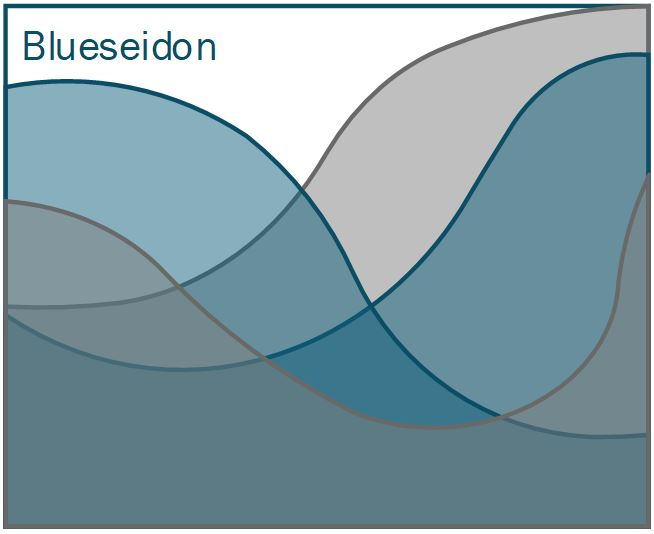
\includegraphics[height=60mm]{images/Blueseidon_Titelbild}
       % \graphicscaption{Ender 3 Pro}
    \end{minipage}%
    \begin{minipage}{0.5\textwidth}
        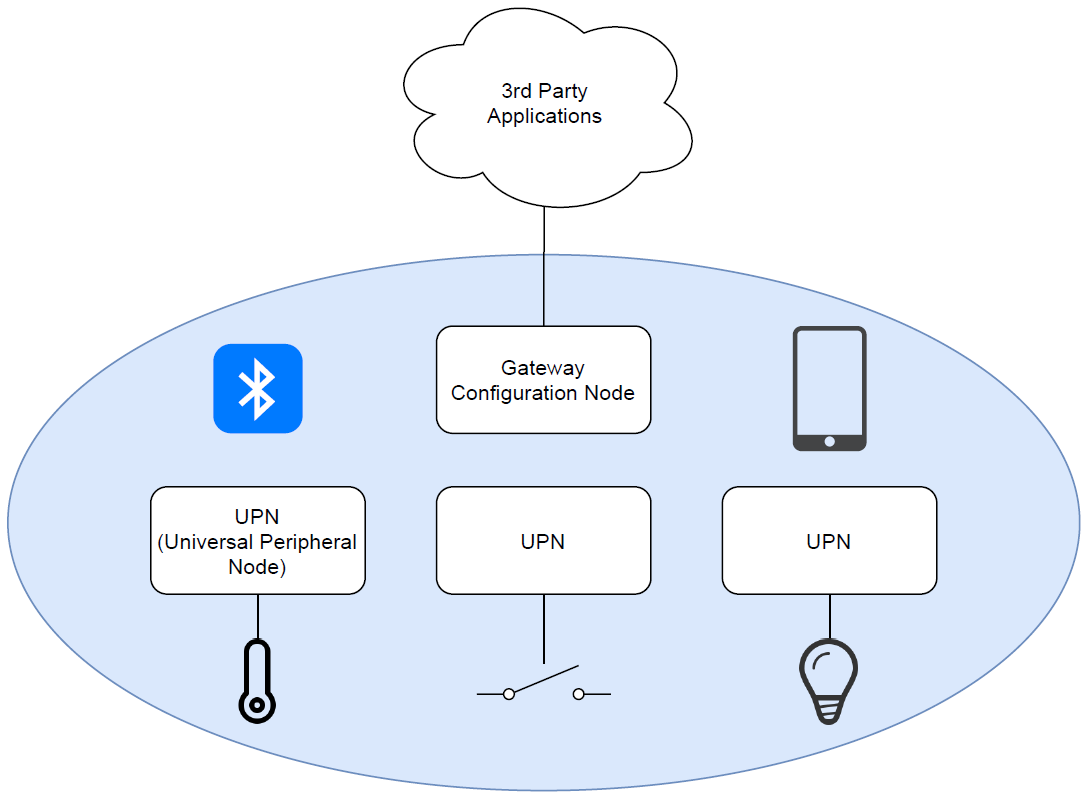
\includegraphics[height=60mm]{images/Grobkonzept_Schema.PNG}
        %\graphicscaption{Grobkonzept}
    \end{minipage}
}

\fscontent{
    \section{Bluetooth Mesh}
    Der von der \textit{Bluetooth SIG (Special Interest Group)} veröffentlichte \textit{Bluetooth Mesh Standard} ermöglicht es, Netzwerkteilnehmer zu einem stark vermaschten Netz zusammenzufassen. Man spricht von einer m:m (many to many)
Topologie. Dies bedeutet das jeder Teilnehmer mit Jedem kommunizieren kann. Der Standard basiert auf \textit{Bluetooth Low Energy (BLE)} und ist somit mit allen Geräten kompatibel die BLE unterstützen. Dies macht \textit{Bluetooth Mesh} zu einem der zurzeit interessantesten Mesh Standards.

    \section{Blueseidon Mesh}
  	In diesem Projekt ist ein eine \textit{Bluetooth Mesh Plattform} entstanden, die es ermöglicht ein Bluetooth Mesh Netzwerk vereinfacht aufzubauen und zu konfigurieren. Die Plattform bietet dem Endanwender die Möglichkeit eine beliebige Anzahl Knoten einzubinden und diese je nach Anwendung zu konfigurieren. Die einzelnen Knoten sind dabei universell gestaltet, sodass beliebige Hardware damit bedient werden kann. Jeder Node kann als Sensor oder Aktor mit analoger oder digitaler Peripherie eingesetzt werden.
  	
  	\section{Energy Harvesting}
	Ein Ziel dieses Projektes ist es die Bluetooth Mesh Knoten möglichst netzunabhängig zu betreiben. Dazu sollte sogenanntes Energy Harvesting eingesetzt werden. Energy Harvesting steht als Überbegriff für die Energiegewinnung aus der Umgebung, wozu beispielsweise Solarenergie, Vibrationsenergie, Thermische Energie aber auch die Energie von Elektromagnetischen Wellen zählt. Um für jede Anwendung die passende Energy-Harvesting Methode zu evaluieren wurde ein Machbarkeitsstudie durchgeführt. Darin hat sich gezeigt, dass der Einsatz solcher Methoden tatsächlich möglich wäre, wobei allerdings die Bedingungen oft beinahe ideal sein müssten. Einzig die Solarenergie könnte wohl verbreitet eingesetzt werden.

    \section{Node-Red Dashboard}
    Um dem Benutzer eine einfache und praktikable Bedienoberfläche zu bieten wird eine \textit{Node-Red} Dashboard eingesetzt. \textit{Node-Red} basiert auf \textit{JSON} und \textit{Java-Script} und läuft auf einem \textit{Raspberry-Pi} Minicomputer welcher künftig auch als Gateway eingesetzt werden soll. Zusammen mit eine \textit{Python} Script und dem \textit{nRF52840 Development Kit} als Hardwareschnittstelle wird der Raspberry-Pi zu einem Bluetooth Mesh Knoten und kann das Netz verwalten und steuern.\\



   \begin{minipage}{0.6\textwidth}
   	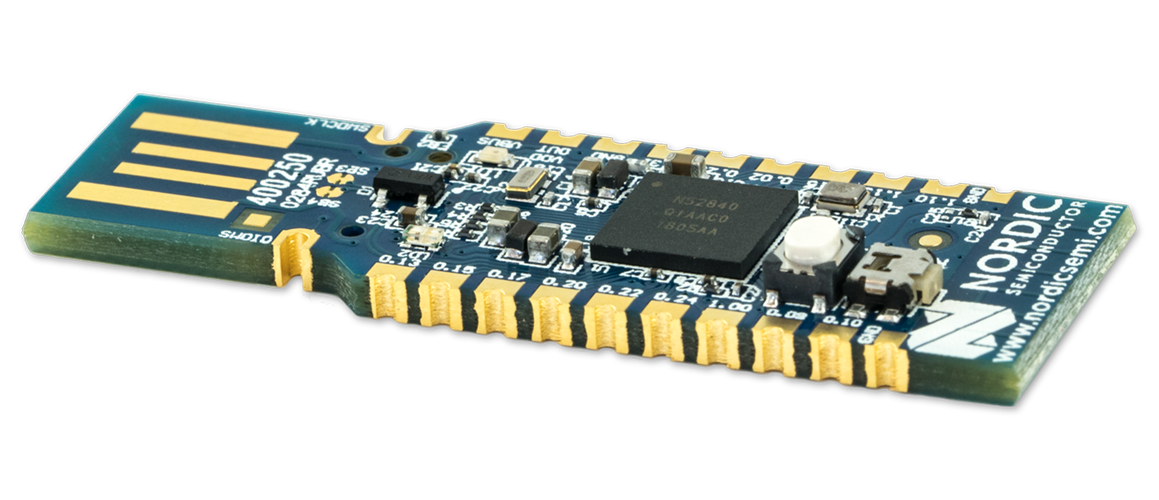
\includegraphics[height=25mm]{images/nRF52840_Dongle.png}
   \end{minipage}
}

\infobox{Highlights}{%
    \footnotesize
    \setlength\tabcolsep{2pt}
   	\begin{itemize}
   	\item nRF52840
   	\item Bluetooth Mesh
   	\item Node-Red
	\end{itemize}
}
